% ---------------------------------------------------------------------------
% Author guideline and sample document for EG publication using LaTeX2e input
% D.Fellner, v1.13, Jul 31, 2008

\documentclass{egpubl}
\usepackage{eurovis2018}
\usepackage{subcaption}
\Full_EuroVis
% --- for  Annual CONFERENCE
% \ConferenceSubmission   % uncomment for Conference submission
%\ConferencePaper        % uncomment for (final) Conference Paper
% \STAR                   % uncomment for STAR contribution
% \Tutorial               % uncomment for Tutorial contribution
% \ShortPresentation      % uncomment for (final) Short Conference Presentation
% \Areas                  % uncomment for Areas contribution
% \MedicalPrize           % uncomment for Medical Prize contribution
% \Education              % uncomment for Education contribution
%
% --- for  CGF Journal
% \JournalSubmission    % uncomment for submission to Computer Graphics Forum
% \JournalPaper         % uncomment for final version of Journal Paper
%
% --- for  CGF Journal: special issue
% \SpecialIssueSubmission    % uncomment for submission to Computer Graphics Forum, special issue
\SpecialIssuePaper         % uncomment for final version of Journal Paper, special issue
%
% --- for  EG Workshop Proceedings
% \WsSubmission    % uncomment for submission to EG Workshop
% \WsPaper         % uncomment for final version of EG Workshop contribution
%
 \electronicVersion % can be used both for the printed and electronic version

% !! *please* don't change anything above
% !! unless you REALLY know what you are doing
% ------------------------------------------------------------------------

% for including postscript figures
% mind: package option 'draft' will replace PS figure by a filname within a frame
\ifpdf \usepackage[pdftex]{graphicx} \pdfcompresslevel=9
\else \usepackage[dvips]{graphicx} \fi

\PrintedOrElectronic

% prepare for electronic version of your document
\usepackage{t1enc,dfadobe}

\usepackage{egweblnk}
\usepackage{cite}
\usepackage{cleveref}
\usepackage{amsmath}


% For backwards compatibility to old LaTeX type font selection.
% Uncomment if your document adheres to LaTeX2e recommendations.
% \let\rm=\rmfamily    \let\sf=\sffamily    \let\tt=\ttfamily
% \let\it=\itshape     \let\sl=\slshape     \let\sc=\scshape
% \let\bf=\bfseries

% end of prologue

\title[EG \LaTeX\ Author Guidelines]%
{Progressive data streams}

% for anonymous conference submission please enter your SUBMISSION ID
% instead of the author's name (and leave the affiliation blank) !!
\author[D. Fellner \& S. Behnke]
{D.\,W. Fellner\thanks{Chairman Eurographics Publications Board}$^{1,2}$
  and S. Behnke$^{2}$
  %        S. Spencer$^2$\thanks{Chairman Siggraph Publications Board}
  \\
  % For Computer Graphics Forum: Please use the abbreviation of your first name.
  $^1$TU Darmstadt \& Fraunhofer IGD, Germany\\
  $^2$Institut f{\"u}r ComputerGraphik \& Wissensvisualisierung, TU Graz, Austria
  %        $^2$ Another Department to illustrate the use in papers from authors
  %             with different affiliations
}

% ------------------------------------------------------------------------

% if the Editors-in-Chief have given you the data, you may uncomment
% the following five lines and insert it here
%
% \volume{27}   % the volume in which the issue will be published;
% \issue{1}     % the issue number of the publication
% \pStartPage{1}      % set starting page


%-------------------------------------------------------------------------
\begin{document}
  
% \teaser{
%  
\includegraphics[width=\linewidth]{eg_new}
%  \centering
%   \caption{New EG Logo}
% \label{fig:teaser}
% }

\maketitle

\newcommand{\norm}[1]{\left\lVert#1\right\rVert}
\begin{abstract}
Performing scientific analysis on the petabytes of data commonly found nowadays is an onerous task
due to the prohibitive cost of data transfer. Currently this issue is alleviated by working with
reduced-resolution or reduced-precision data. This paper brings together techniques that reduce data
in resolution, precision, and both, into a common framework in which they can be studied and
compared. Their error patterns are compared with regards to fundamental metrics, namely L2 norm,
first and second derivatives, histograms, and isocontours. We also compute and study
metric-dependent, data-optimal streams which serve as empirical bounds on the limit to which
reduction can happen, given an error tolerance for the analysis task at hand. Finally, based on the
observed characteristics of those streams, we propose practical heuristics to minimize the amount of
data needed to perform a given analysis task. The insights and heuristics presented here can be
leveraged to implement data-optimal representations and querying systems to facilitate interactive
exploration as well as cursory analysis of enormous data.  
\begin{classification} % according to http://www.acm.org/class/1998/
  \CCScat{Computer Graphics}{I.3.3}{Picture/Image Generation}{Line and curve generation}
\end{classification}
  
\end{abstract}

%\input{EGauthorGuidelines-body.inc}
As the gap between the available compute power and the cost of data movement increases, data
transfer, whether from cache, main memory, or from disk, becomes a major bottleneck in many
workflows. However, it has been shown that not every bit of data is always necessary to answer
scientific questions with required accuracy. In particular, for techniques at the end of scientific
workflows, such as visualization and data analysis, lower fidelity representations of the data often
provide adequate approximations~\cite{woodring2011,covra2012,compression_sim2013}, and even during
simulation some loss in precision is often
acceptable~\cite{compression_sim2013,doi:10.1177/1094342018762036}. As a result, several different
techniques have been proposed to reduce the size of data. 

Broadly, these techniques can be classified into (i) reducing the data resolution, e.g., the number
of data points stored, and (ii) reducing the precision of each data point. Examples of the former
kind of approaches are subsampling~\cite{idx2001}, adaptive mesh refinement~\cite{amr1989}, octrees
and other tree structures~\cite{hierarchical1984}, and wavelets~\cite{woodring2011}, and those of
the latter are various forms of
compression~\cite{fpzip,isabela,zfp2014,sz,vq1992,compression_domain2003,sqe}. Traditionally,
multiresolution structures have been used to accelerate dynamic queries, e.g., in
rendering~\cite{multires_octree1999}, since discarding data points based on the viewpoint or data
complexity can result in significant speed-up. Compression based on quantization, on the other hand,
is more common when storing data, where in the absence of other information, treating each sample as
equally important is the null hypothesis. However, in many situations, a combination of both
resolution and precision reduction could be appropriate. For example, high spatial resolution may be
needed to resolve the topology of an isosurface, yet the corresponding data samples may be usable at
less than full precision to adequately approximate the geometry. Conversely, accumulating accurate
statistics may require high-precision values, yet a lower resolution subset of data points may be
sufficient for the task. 

In general, different levels of adaptivity in combinations of resolution and precision may be
suitable for different types of analysis and visualization tasks, and for many, these requirements
will be data dependent. Consequently, a globally optimal data organization may not exist. Instead,
we consider a progressive setting in which some initial data is loaded and processed, and new data
is requested selectively based on the requirement of the current task as well as the characteristics
of the data already loaded. The result is a stream of bits ordered such that the error is minimized,
considering the task at hand. However, although intuitively there are almost certainly advantages in
considering both resolution and precision in the ordering, it is unclear how much the error could be
reduced for a given data budget or how little data could be used to achieve the same error.
Furthermore, optimal data-dependent orderings may be especially impractical since they assume
perfect knowledge of the data. It is therefore important to understand which of these potential
gains are realizable. This paper aims to answer these important questions about the suitable bit
orderings through extensive, empirical experiments. In particular, this paper presents:

\begin{itemize}\dense
%
\item a framework that allows systematic studies of the resolution-versus-precision tradeoffs for
common data analysis and visualization tasks. The core idea is to represent various data reduction
techniques as bit streams that improve data quality in either resolution or precision in each step
(\Cref{sec:terminologies}). We can thus compare these techniques fairly, by comparing the
corresponding data streams.
%  
\item empirical evidence that jointly optimizing resolution and precision can provide significant
improvements on the results of analysis tasks over adjusting either independently. 
We present a diverse collection of data sets and data analysis tasks, and also show how
different types of data analysis might require substantially different data streams for optimal
results.
%
\item a greedy approach that gives estimations for lower bounds of error for various analysis tasks.
In addition, we also identify practical streams that closely approximate these bounds for each task
(\Cref{sec:rmse-optimized}, \Cref{sec:derivatives}, \Cref{sec:histogram}, and
\Cref{sec:isocontour}), using a novel concept called \emph{stream signature}
(\Cref{sec:stream-signature}), which is a small matrix that captures the essence of how a bit stream
navigates the precision-versus-resolution space.
\end{itemize}


%%% Local Variables:
%%% mode: latex
%%% TeX-master: "template"
%%% End:

\section{Related work}

\para{Tree-based multiresolution hierarchies.}
Techniques that reduce data in resolution typically build a tree-shape hierarchy over the data. A
very common scheme to generate such a hierarchy is to construct low-resolution copies of the data
from higher resolution ones through filtering or subsampling. Examples include Gaussian and
Laplacian pyramids~\cite{laplacian-pyramid},
mipmaps~\cite{multires_octree1999,interactive-exploration-ct-scans}. Often, the data is stored in
blocks on each resolution level. To save bandwidth, low-resolution blocks can be streamed during
rendering, if the points being queried project to less than a pixel on screen. However, these
methods increase storage requirements and potentially expensive pre-processing, making them
unsuitable for very large data.

Recent multi-resolution techniques save storage by adapting to the data in such a way that different
regions of the data are stored in different resolutions and depending on how ``homogeneous'' is the region.
Fast-varying regions are stored at higher resolution. A very popular approach is sparse voxel
octrees (SVO), pioneered by Crassin \etal~\cite{gigavoxels} and Gobbetti \etal~\cite{Gobbetti2008},
and variations of which are found in~\cite{Fogal-2013-RayGuided,visualization-driven}. Sparsity
comes from the fact that smooth-varying regions are stored at coarser octree levels, which
significantly reduces storage. During rendering, blocks of samples are streamed from an appropriate
resolution, determined by how far the queried samples are from the eye/camera. Beyer
\etal~\cite{large‐scale-volume} give a comprehensive overview of state-of-the-art GPU-based
out-of-core ray-casting techniques.

Beside octrees, other trees such as B+ tree~\cite{vdb2013} and
kd-tree~\cite{fogal-kdtree,in-situ-sampling-particle} can also be used to build a sparse hierarchy.
Alternatively, space-filling curves such as the hierarhical Z curve~\cite{idx2001} or the Hillbert
curve~\cite{mloc} can be used to reorder data samples to form a hierarchy without any filtering
steps or redundant samples, as low-resolution levels are constructed via subsampling. Unfortunately,
subsampling can introduce aliasing.

%\paragraph{\textbf{Transform-based multiresolution hierarchies}}
\para{Transform-based multiresolution hierarchies.}
Other multiresolution approaches reduce data by transform-based compression. For example,
COVRA~\cite{covra2012} constructs an octree of bricks, each of which is further subdivided \pavol{into?} blocks.
Compression is done by learning a sparse representation for the blocks in terms of prototype (basis)
blocks. Similarly, Fout\etal~\cite{hw_dvr2007} transform each block in the volume using the KLT
transform, which produces several classes of partitions (each can be thought of as one resolution
level). They compress the transform coefficients using vector quantization~\cite{vq1992} by
constructing one codebook for each paritition class. Schneider~\etal~\cite{compression_domain2003}
also use vector quantization on transform coefficients, but with a simple Haar-like transform that
separates each block of $2^3$ voxels into one average and seven difference coefficients.

Analogous to the KLT transform in 2D, the Tucker decomposition~\cite{tensor_dvr2015} in
$n$-dimensional space decomposes the input data (stored as a tensor) into $n$ matrices of basis
vectors and one core tensor. Reduction in storage and in transmission bandwidth comes from the fact
that the basis matrices can be downsampled (resulting in a lower resolution representation) and the
core tensor can be rank-truncated (resulting in coarse-scale representations of
features)~\cite{tamresh,tucker-thresholding,multiscale-tensor}. Furthermore, elements in the basis
matrices and the core tensor can be thresholded~\cite{tucker-thresholding} or
quantized~\cite{tamresh,multiscale-tensor}. Tensor decomposition can work for higher dimensional
data and can achieve very high compression ratios. However, the transform step is costly due to it
being data-dependent.

%\paragraph{\textbf{Wavelets}}
\para{Wavelets.}
Transforms that use fixed bases avoid such high computation cost at the expense of slightly less
effective compression. Perhaps the most popular transform that uses a fixed basis is the (discrete)
wavelet transform (DWT). The DWT constructs a hierarchy of resolution levels via low and high
bandpass filters. The transform is recursively applied to the lower resolution band, resulting in a
hierarchy of ``details'' at varying resolution. One benefit of wavelets over redundant
representations such as Laplacian pyramids is that the wavelet transform is merely a change of basis
that like reordering techniques does not increase the data size. Another benefit over adaptive
refinement meshes and other tree-like techniques is that the wavelet basis functions are defined
everywhere in space, requiring no special interpolation rules when given some arbitrary subset of
wavelet coefficients and basis functions. One disadvantage of the wavelet transform is the random
access cost, which is not constant time. However, there has been work to develop acceleration
structures to speed up local queries~\cite{weiss}.

Beside offering a multiresolution decomposition, enabling data streaming with level-of-detail
support, wavelets also offer ample opportunities for compression. As the magnitude of wavelet
coefficients decays rapidly for a typical volume [CITE], they are especially amenable to thresholding
or entropy compression. In the context of storing and visualizing scientific data, wavelets (with
compression) are used in a wide variety of
systems~(\cite{multires_toolkit2003,vapor2007,woodring2011}) and applications (volume rendering
with
level-of-detail~\cite{wavelet-compression-interactive-vis,multires-framework,rapid-compression-volume,interactive-rendering-large-volume,multires-volume-rendering},
turbulence visualization~\cite{treib}, particle visualization~\cite{sph-octree}).

Most wavelet-based techniques employ tiling of wavelet coefficients in individual subands to
facilitate random access and spatial adaptivity in resolution. For example, the VAPOR
toolkit~\cite{vapor2007} incorporates a multiresolution file format based on a wavelets to allow
data analysis on commodity hardware by storing individual tiles in separate files to allow loading
of the region of interest. However, like most multiresolution work, only the resolution control is
leveraged. The precision axis, which can potentially further reduce data transfer, is left
unexplored.

%\paragraph{\textbf{Wavelet coders}}
\para{Wavelet coders.}
Most work that explores the precision axis comes from state-of-the-art coders for wavelet
coefficients in image compression. Wavelet coefficients in corresponding regions across subbands can
be thought of as belonging to a ``tree'', with the root being a single coefficient at the lowest
subband. Thee emmbedded zerotrees (EZW) coder exploits the property that in such trees, ``parent''
coefficients are often larger in magnitude than ``child'' coefficients. It locates trees of wavelet
coefficients that are insignificant with regard to (i.e., less than in magnitude) a threshold. Such
a tree is encoded with one single symbol, resulting in significant compression. The threshold is
typically set at each bit plane, starting from the most significant one. In this way, the data can
be progressively refined in precision during decompression. The SPIHT coder~\cite{spiht1996}
improves on EZW by locating more general types of zero trees~\cite{quantifying-coding-performance}.
SPECK~\cite{speck2004} extends SPIHT to exploit also spatial correlations among nearby coefficients
on the same subband.

%\paragraph{\textbf{Floating-point compression}}
\para{Floating-point compression.}
\newcommand{\zfp}{\textsc{zfp}\xspace}
The \zfp compression scheme~\cite{zfp2014} also encodes transform coefficients by bit plane, in
order of decreasing significance. \zfp partitions the domain---a structured grid---into small (e.g.,
$4 \times 4 \times 4$) independent blocks and thus allows for localized decompression. Moreover,
\zfp supports fixed-rate compression that facilitates random access to the data. Its fast transform
and caching of decompressed data allows it to achieve not only high throughput decompression, but
also fast inline compression. Extensions of \zfp allow it to vary either the bit rate or precision
spatially over the domain, albeit at fixed resolution~\cite{zfp-arc}. Other notable compression
schemes for scientific data include scalar quantization encoding (SQE)~\cite{sqe},
ISABELA~\cite{isabela}, SZ~\cite{sz}, and FPZIP~\cite{fpzip}. The latter three employ prediction and
compress the residuals. ISABELA and SZ perform residual scalar quantization, whereas FPZIP truncates
floats, which can be seen as nonuniform scalar quantization. Similar to FPZIP, the precision-based
level of details (PLoD) scheme proposed in MLOC~\cite{mloc} also truncates floats by dividing a
double-precision number into seven parts, of which the first part contains the first two bytes, and
each of the other six parts contains one byte for additional precision. MLOC includes a
multiresolution scheme based on Hillbert curves, but this scheme (based on resolution) and the PLoD
scheme (based on precision) are exclusive.

%\paragraph{\textbf{Mixing resolution and precision}}
\para{Mixing resolution and precision.}
Schemes that allow progressive data access in both resolution and precision include
SBHP~\cite{sbhp2000} and JPEG2000~\cite{jpeg2000}. Both partition each subband into blocks and code
each block independently, in bit plane order. By interleaving compressed bits across blocks, one can
construct a purely resolution-progressive or a purely precision-progressive stream, or anything in
between. Outside image compression, JPEG2000 has found use in the compression of scientific data. For
example, Woodring \etal~\cite{woodring2011} use JPEG2000 to store floating point data. Since most
JPEG2000 implementations are limited to integer data, the authors apply uniform scalar quantization
to convert floating point data to integer form. Even though JPEG2000 supports varying both
resolution and precision, the authors do not explore this capability but focus only on setting bit
rate. In general, although there exist mechanisms that simultaneously leverage both axes of data
reduction, especially for the purpose of scientific data analysis, they have not been
well-studied.

%\paragraph{\textbf{Error quantification}}
\para{Error quantification.}
Several works have aimed at quantifying the error incurred by data reduction, by
compression or otherwise, for the results of analysis tasks. Baker
\etal~\cite{evaluating-compression-climate} evaluate several compressors (FPZIP~\cite{fpzip},
APAX~\cite{apax}, ISABELA~\cite{isabela}) on ensembles of climate simulation data, using the
root-mean-square z-score (RMSZ) as the error metric. Laney \etal~\cite{compression_sim2013} study
the effects of lossy compression (using FPZIP and APEX) on the Miranda hydrodynamic simulation code,
using physics-based error metrics. Li \etal~\cite{evaluating-efficacy-wavelet} measure the error
incurred by wavelet compression on turbulent-flow data, using root-mean-square error of
radial-enstrophy profiles as the metric. Wang \etal~\cite{statistical-volume-quality} assess the
quality of distorted data using a combination of statistical metrics in the wavelet transform
domain. Etiene \etal have published a series of studies on verification of isosurfaces in
geometrical~\cite{verifiable-isosurface} and topological~\cite{topology-verification-isosurface}
terms, as well as verification of volume-rendered images~\cite{verifying-volume-rendering}. They
focus on order-of-accuracy and convergence analysis, where errors are introduced mostly through
discretization, not necessarily for the purpose of reducing data bandwidth. Finally, the Z-checker
framework~\cite{z-checker} consists of many independent metrics (which are called analysis
``kernels'') to evaluate data quality after lossy compression. The list includes min/max,
distribution, entropy, smoothness, power spectrum, principal component analysis, and
autocorrelation. In general, however, no studies have examined the
resolution-versus-precision tradeoffs, as well as the various orderings of bits in the context of
data analysis and visualization.

%by magnitude streams~\cite{image_compression1992}
% Transfer function adaptive decompression~\cite{tf_decompression2004}

Finally, for surveys of data reduction techniques in general, we refer the readers to the work of
Rodr\'{\i}guez \etal~\cite{state-of-the-art-compressed-volume} and Li \etal~\cite{li2018}.

\section{The advantages of combining resolution and precision}
\label{sec:motivation}

Traditional data reduction techniques work by either truncating the finest few resolution levels, or
truncating the last few low-ordered bits of every sample, but rarely both. In this section, our aim
is to show that significant gain can be achieved when one combines both dimensions, namely
resolution and precision, for data reduction. To do so, for each data set, we construct and compare
three different streams, which use different sorting criteria to sort the same set of chunks in
decreasing order of weights. We will use $W(c)$ to denote a sorting criteria, which is any function
that takes a chunk $c$ and returns its `'weight'' that determines its importance.

We compare the three streams by plotting an error curve for each, with regards to three error
metrics, namely root-mean-square error (Figure \ref{fig:motivation-rmse}), histogram error (Figure
\ref{fig:motivation-histogram}), and isocontour error (Figure \ref{fig:motivation-isocontour}). For
each metric, the function is reconstructed every time a new chunk is received from a stream, then
the relevant quantity (the function itself, its histogram, or an isocontour) is computed from the
reconstructed function, and compared against the same quantity computed from the original (lossless)
function. The definitions of histogram error and isocontour error are discussed in detail in Section
[REF] and Section [REF] respectively.

\begin{figure}[h]
  \centering
	\subcaptionbox{Boiler}
  {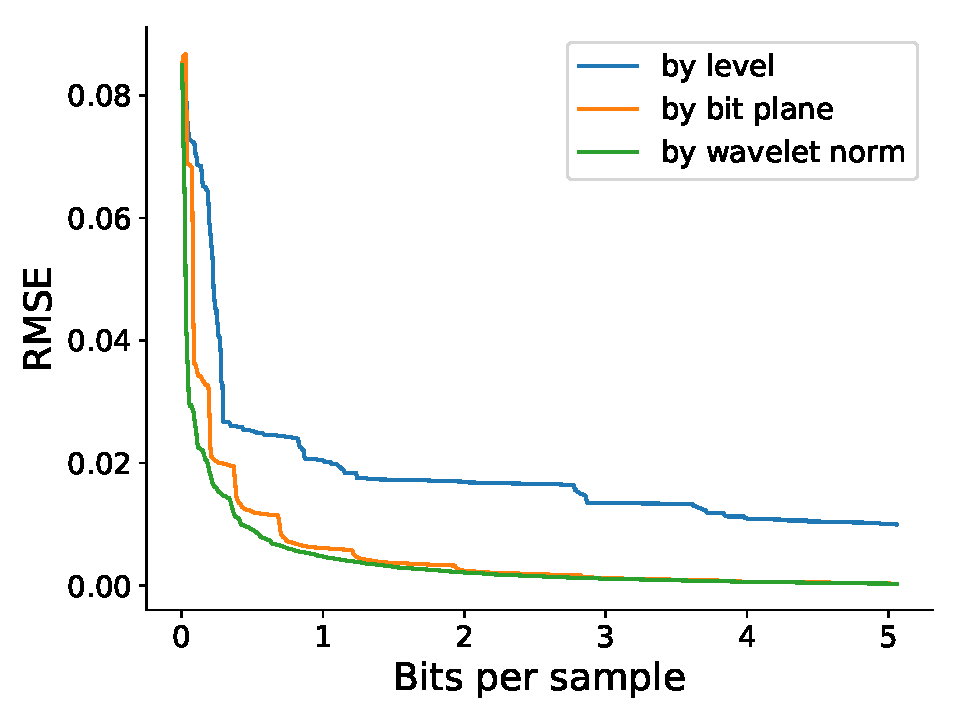
\includegraphics[width=0.48\linewidth]{img/motivation/motivation-psnr-boiler.pdf}}
	\subcaptionbox{Diffusivity}
 	{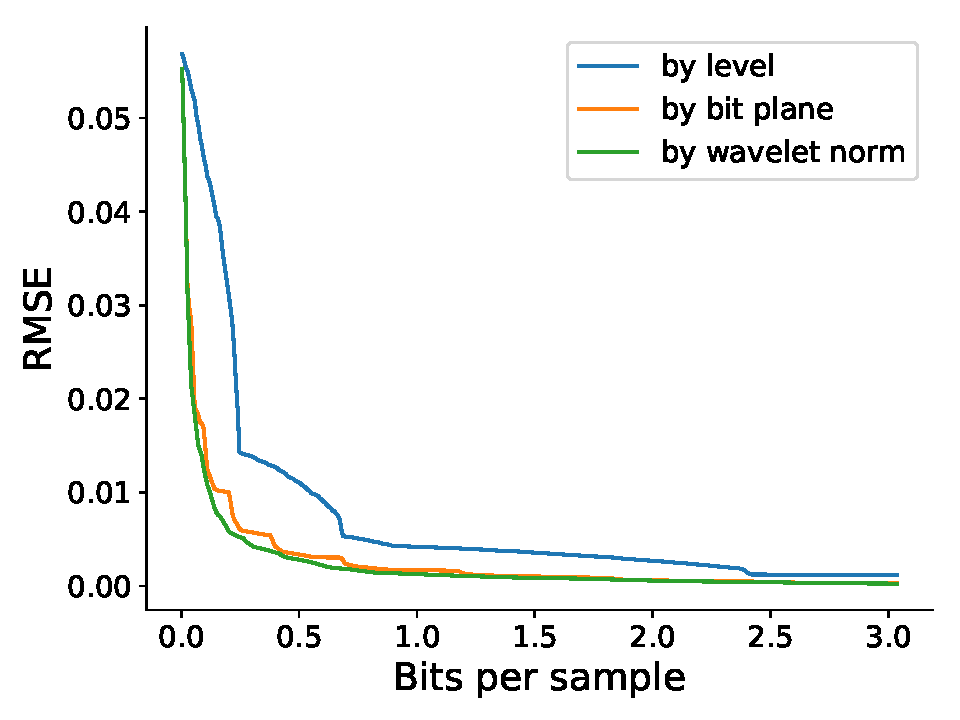
\includegraphics[width=0.48\linewidth]{img/motivation/motivation-psnr-diffusivity.pdf}}
	\subcaptionbox{Euler}
 	{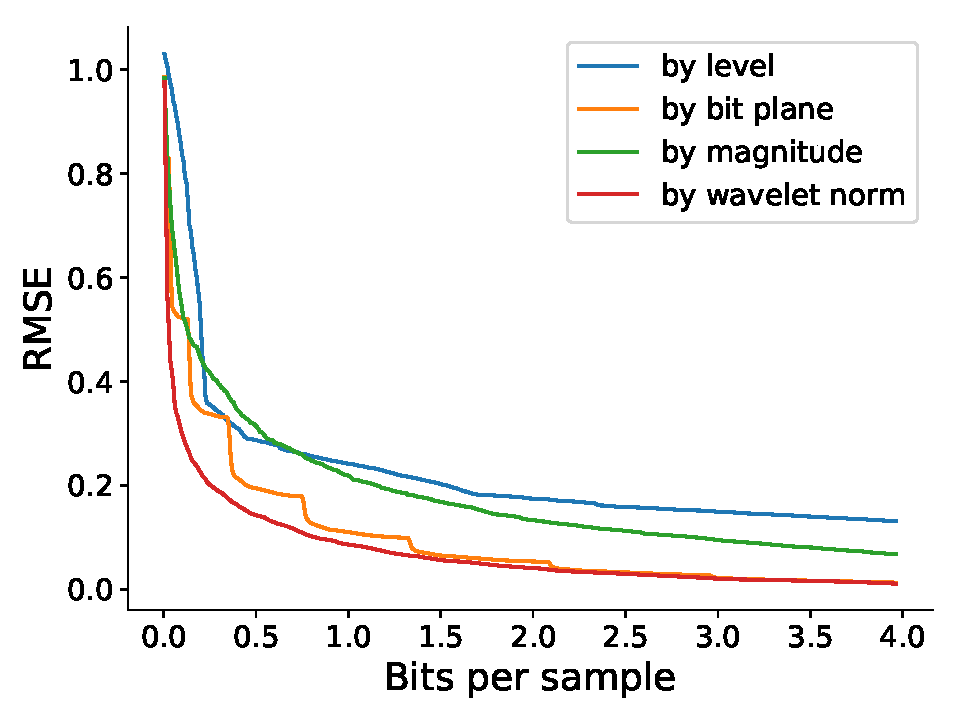
\includegraphics[width=0.48\linewidth]{img/motivation/motivation-psnr-plasma.pdf}}
	\subcaptionbox{Turbulence}
 	{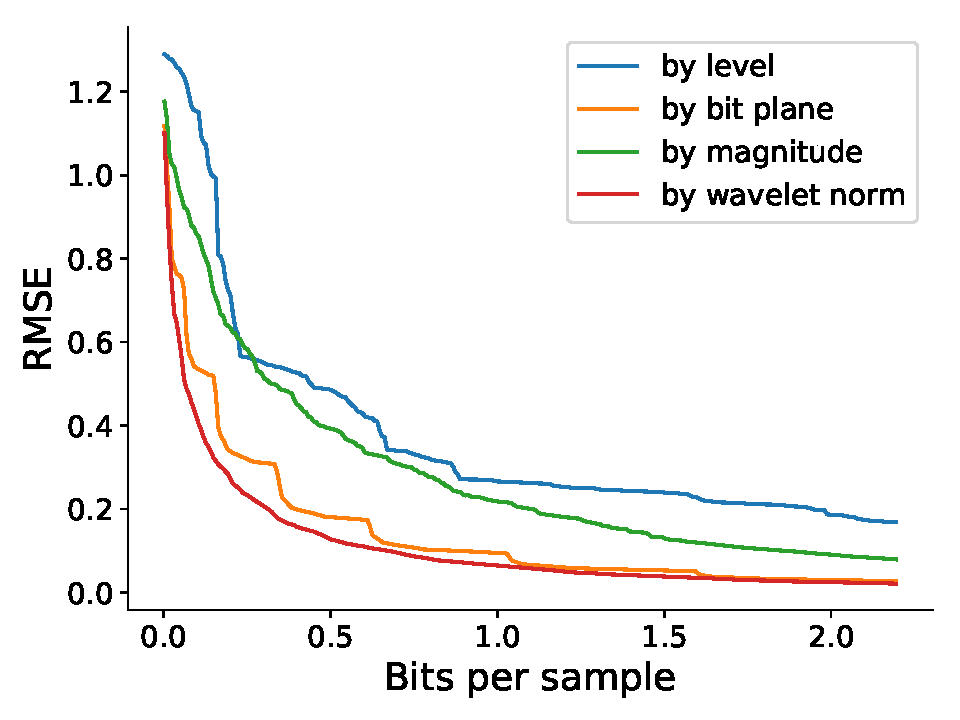
\includegraphics[width=0.48\linewidth]{img/motivation/motivation-psnr-turbulence.pdf}}
	\subcaptionbox{Plasma}
 	{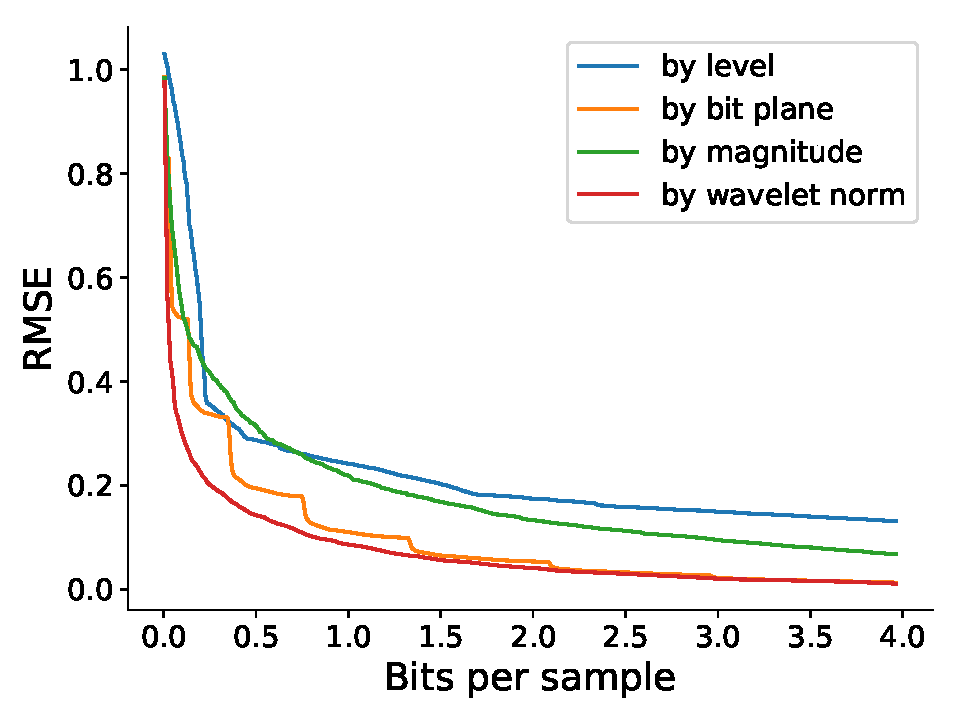
\includegraphics[width=0.48\linewidth]{img/motivation/motivation-psnr-plasma.pdf}}
	\subcaptionbox{Velocity-z}
 	{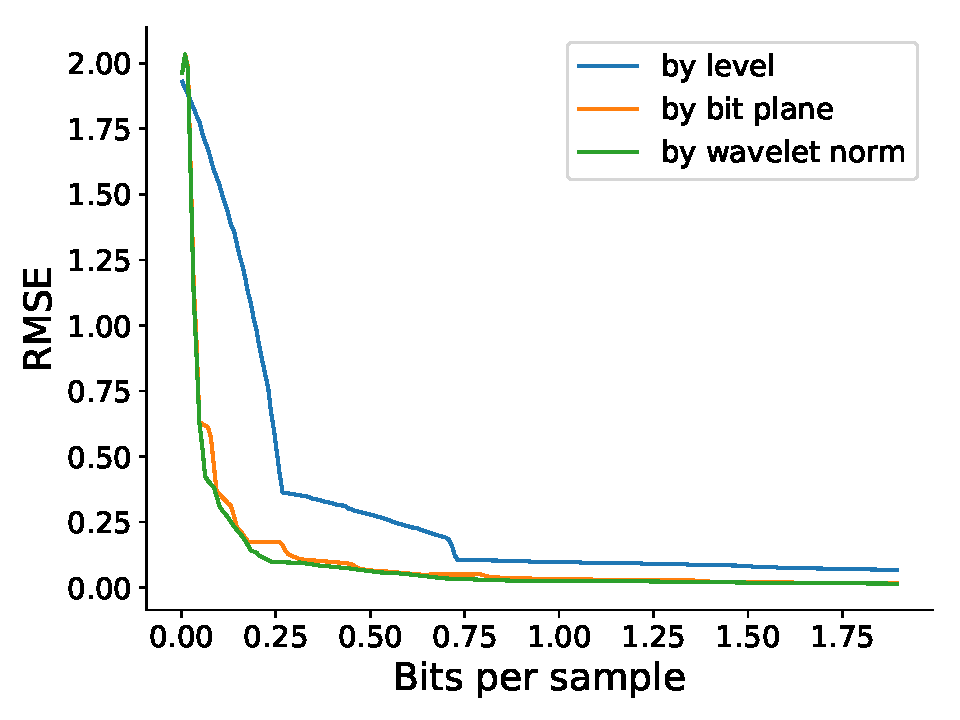
\includegraphics[width=0.48\linewidth]{img/motivation/motivation-psnr-velocityz.pdf}}
 	\caption{Root-mean-square error of reconstructed functions using the three data-agnostic streams
 	defined in Section \ref{sec:motivation}. Lower is better. The streams are truncated to highlight
 	the differences, without omitting important information. \emph{by wavelet norm} performs best,
 	followed closely by \emph{by bit plane}.}
 	\label{fig:motivation-rmse}
\end{figure}

\begin{figure}[h]
  \centering
	\subcaptionbox{Boiler}
  {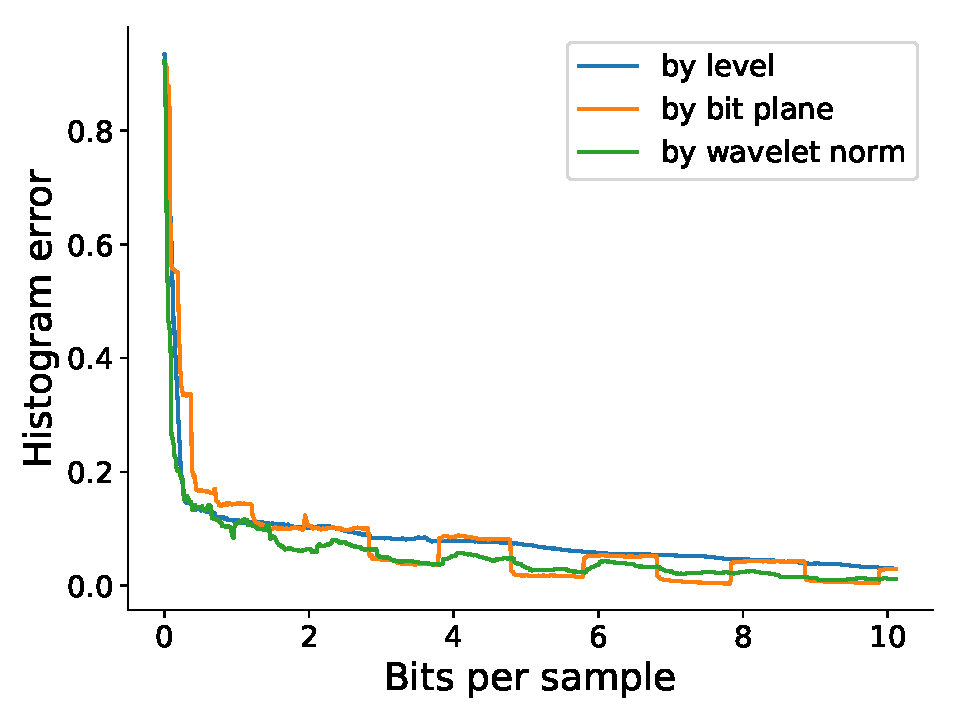
\includegraphics[width=0.48\linewidth]{img/motivation/motivation-histogram-boiler.pdf}}
	\subcaptionbox{Diffusivity}
 	{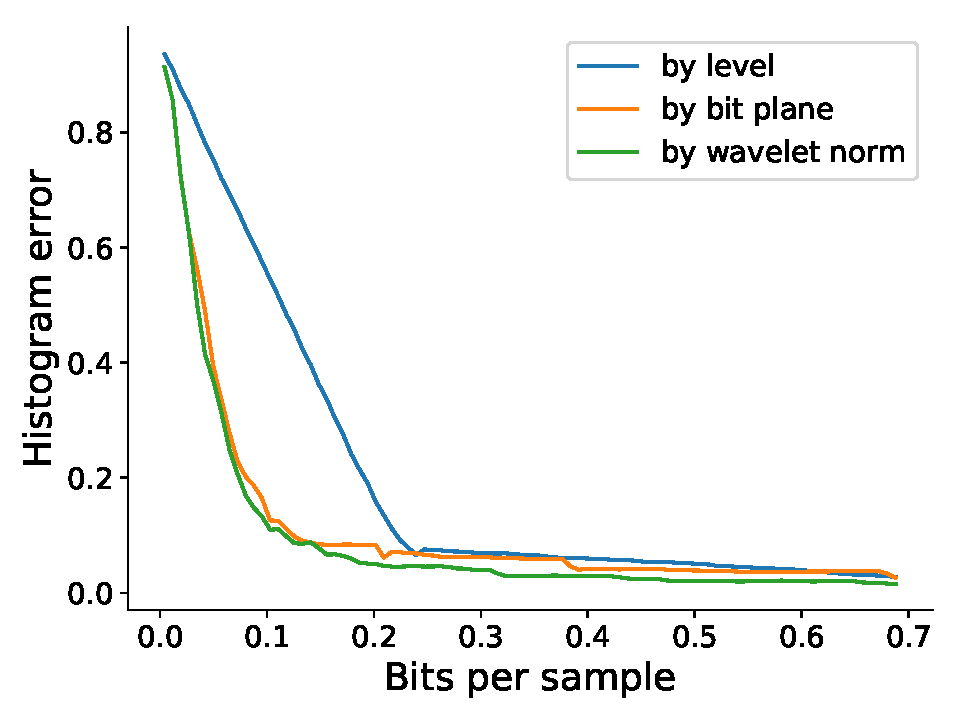
\includegraphics[width=0.48\linewidth]{img/motivation/motivation-histogram-diffusivity.pdf}}
	\subcaptionbox{Euler}
 	{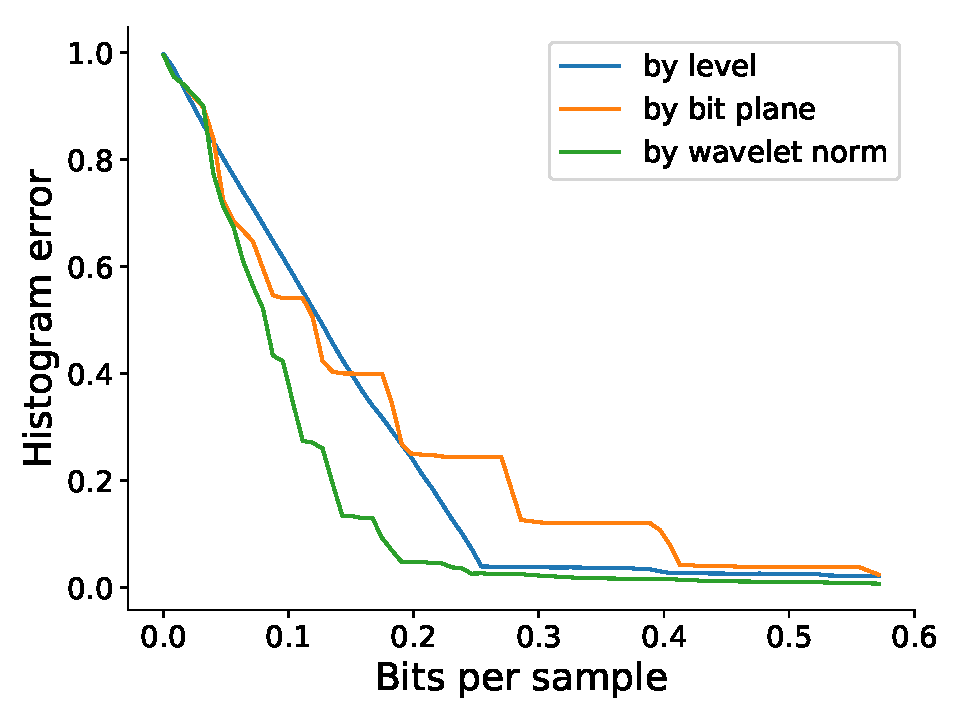
\includegraphics[width=0.48\linewidth]{img/motivation/motivation-histogram-euler.pdf}}
	\subcaptionbox{Turbulence}
 	{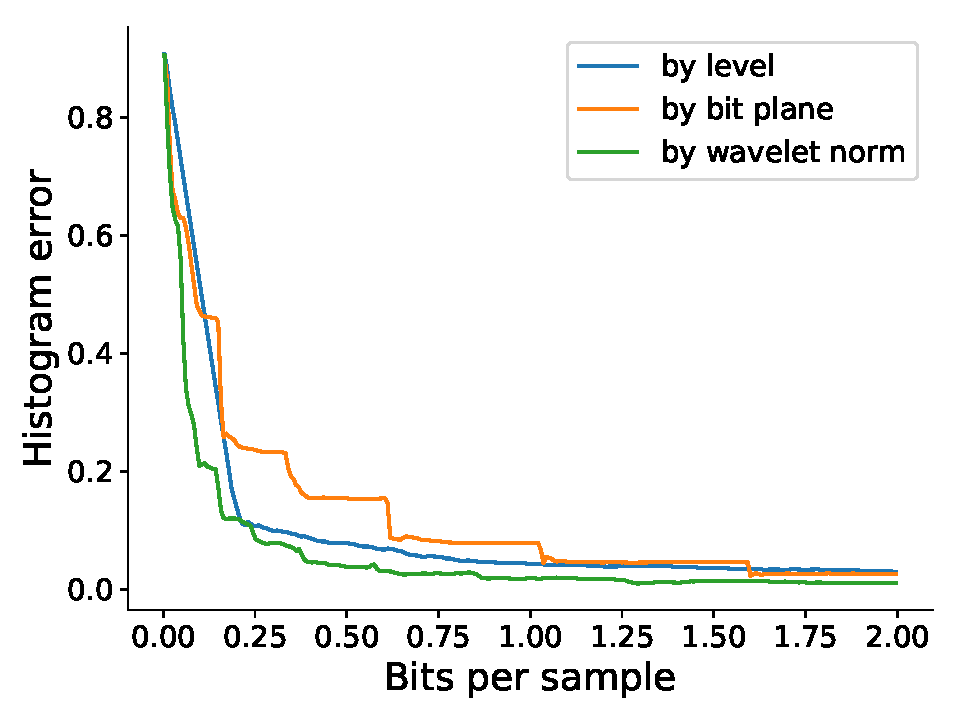
\includegraphics[width=0.48\linewidth]{img/motivation/motivation-histogram-turbulence.pdf}}
	\subcaptionbox{Plasma}
 	{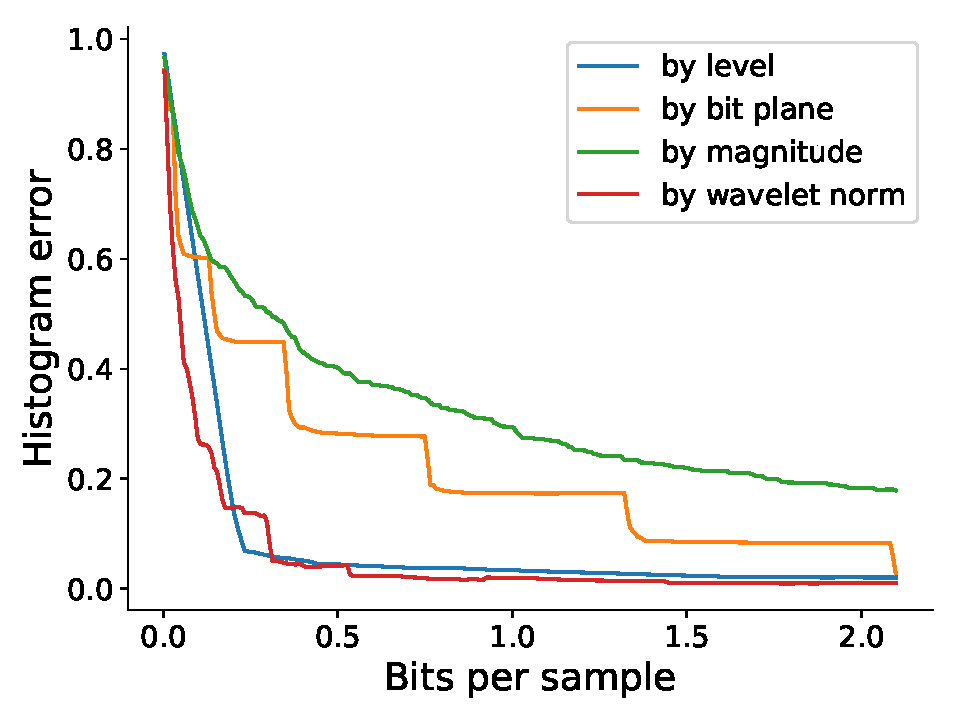
\includegraphics[width=0.48\linewidth]{img/motivation/motivation-histogram-plasma.pdf}}
	\subcaptionbox{Velocity-z}
 	{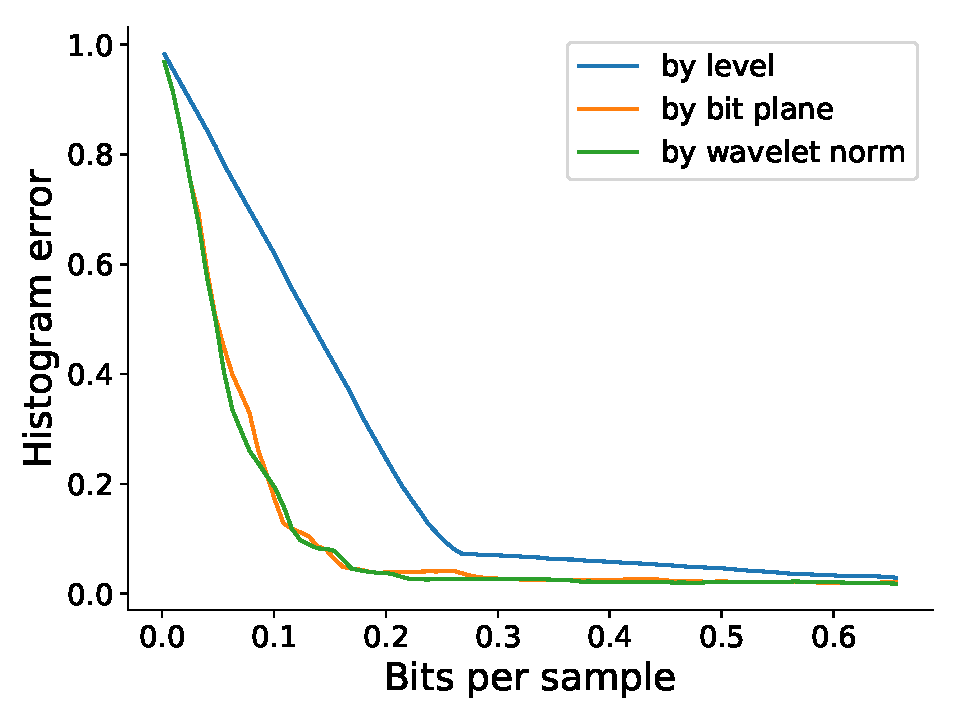
\includegraphics[width=0.48\linewidth]{img/motivation/motivation-histogram-velocityz.pdf}}
 	\caption{Histogram error of reconstructed functions using the three data-agnostic streams defined
 	in Section \ref{sec:motivation}. Lower is better. Each histogram comprises of 256 bins. The
 	streams are truncated to highlight the differences, without omitting important information.
 	\emph{by wavelet norm} performs best.}
 	\label{fig:motivation-histogram}
\end{figure}

\begin{figure}[h]
  \centering
	\subcaptionbox{Boiler, isovalue = $0.07$}
  {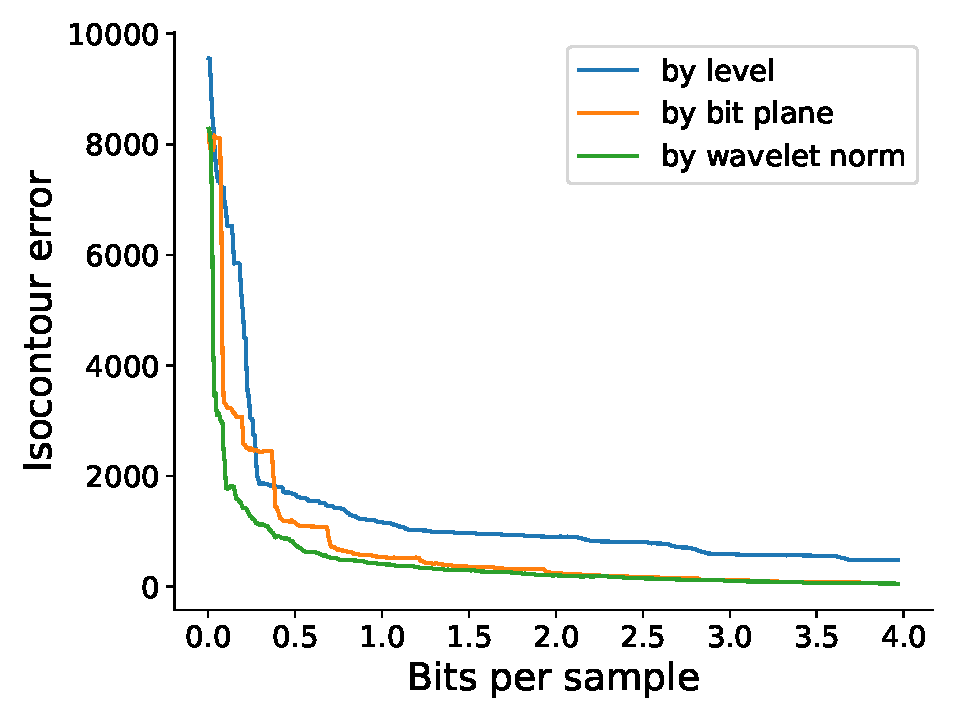
\includegraphics[width=0.48\linewidth]{img/motivation/motivation-isocontour-boiler.pdf}}
	\subcaptionbox{Diffusivity, isovalue = $0.04315$}
 	{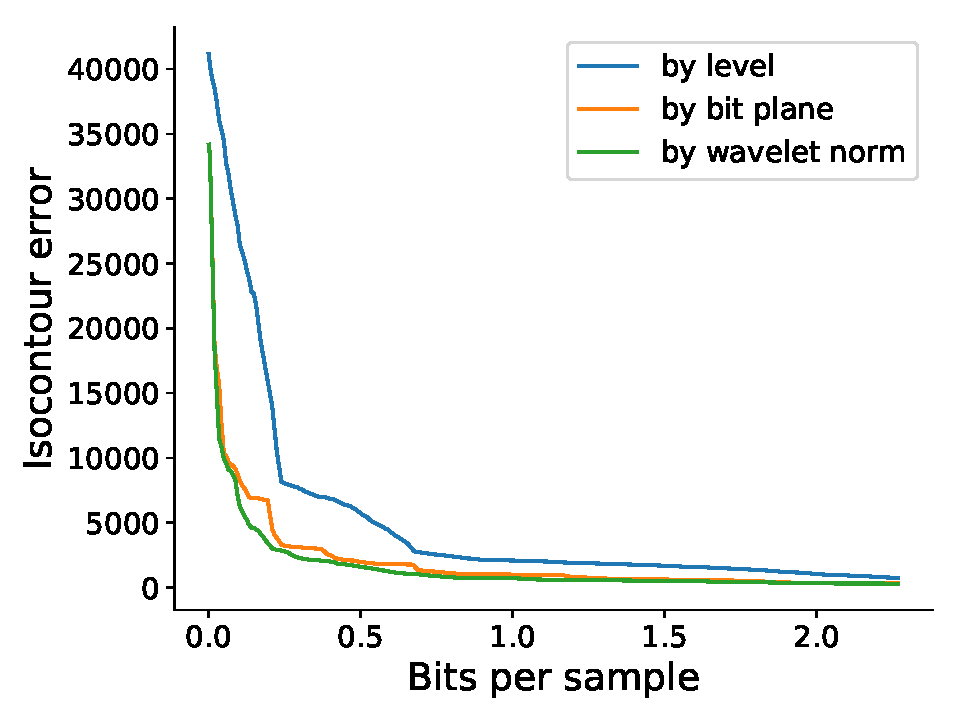
\includegraphics[width=0.48\linewidth]{img/motivation/motivation-isocontour-diffusivity.pdf}}
	\subcaptionbox{Euler, isovalue = $3$}
 	{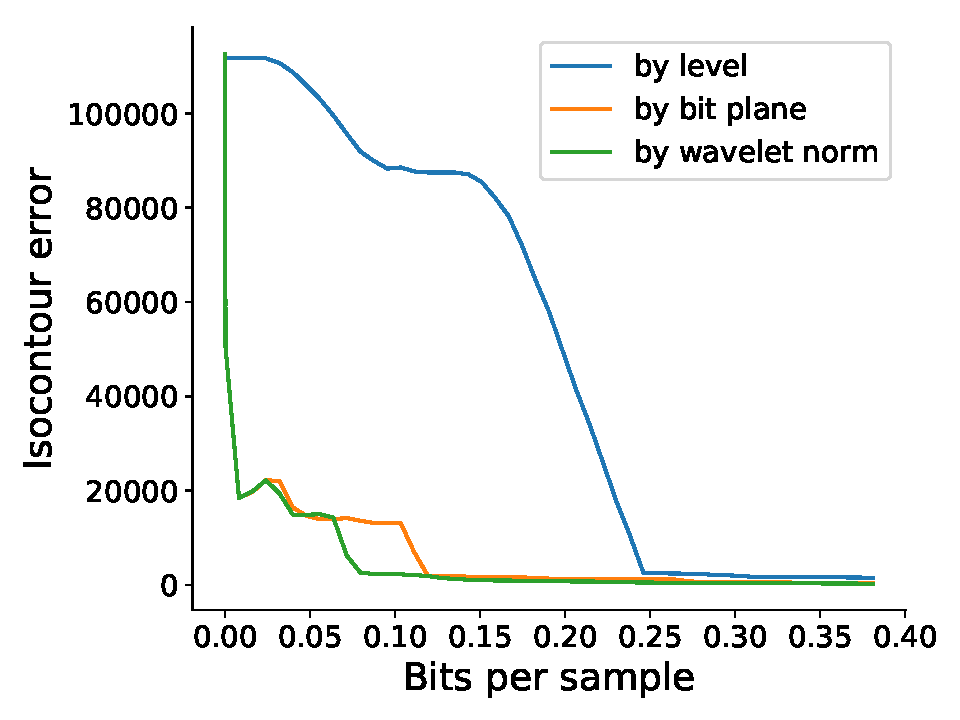
\includegraphics[width=0.48\linewidth]{img/motivation/motivation-isocontour-euler.pdf}}
	\subcaptionbox{Turbulence, isovalue = $2$}
 	{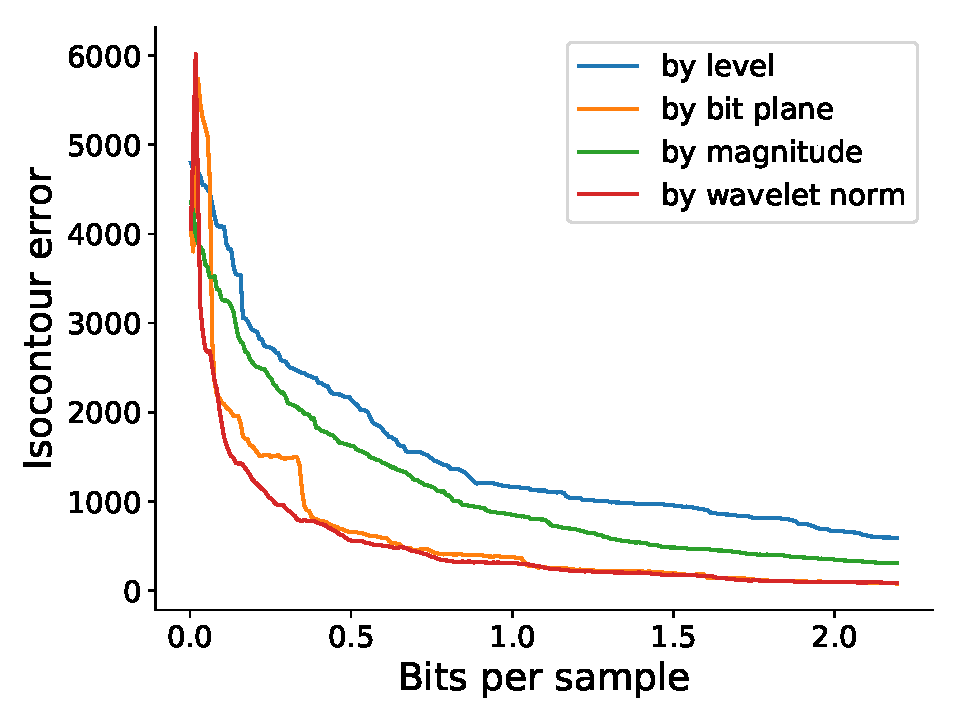
\includegraphics[width=0.48\linewidth]{img/motivation/motivation-isocontour-turbulence.pdf}}
	\subcaptionbox{Plasma, isovalue = $2$}
 	{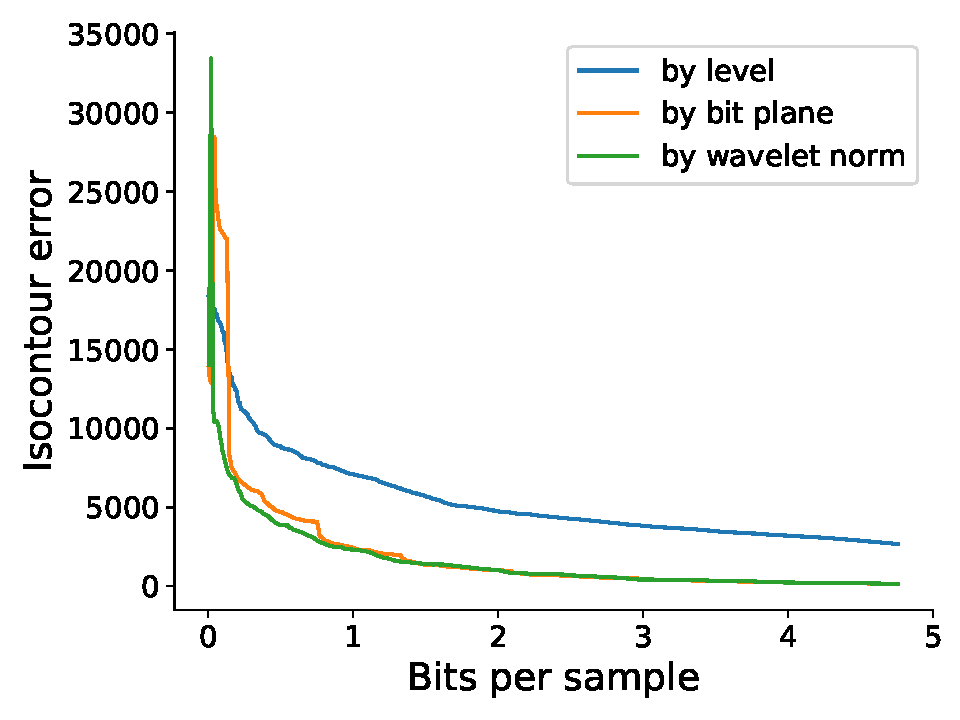
\includegraphics[width=0.48\linewidth]{img/motivation/motivation-isocontour-plasma.pdf}}
	\subcaptionbox{Velocity-z, isovalue = $-2$}
 	{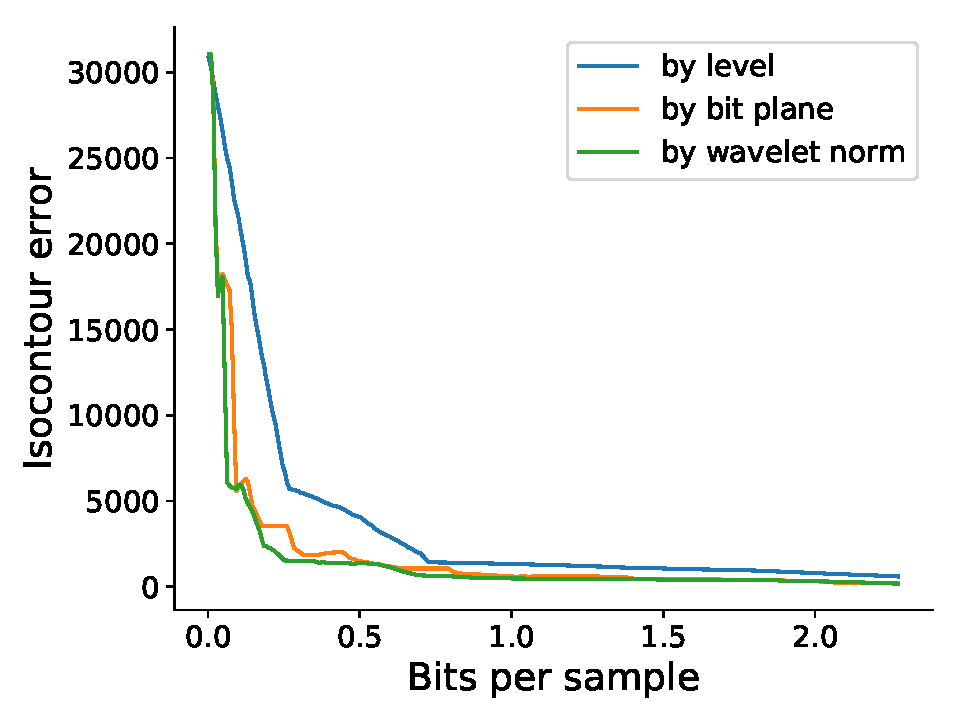
\includegraphics[width=0.48\linewidth]{img/motivation/motivation-isocontour-velocityz.pdf}}
 	\caption{Isocontour error of reconstructed functions using the three data-agnostic streams defined
 	in Section \ref{sec:motivation}. Lower is better. The streams are truncated to highlight the
 	differences, without omitting important information. \emph{by wavelet norm} performs best.}
 	\label{fig:motivation-isocontour}
\end{figure}

We see that, for all metrics, the \emph{by wavelet norm} stream consistently performs the
best. The \emph{by bit plane} works almost as well as \emph{by wavelet norm} for RMS error and
isocontour error, but not for histogram error. The \emph{by level} stream works poorly in almost all cases.
These results show that it is often suboptimal to stream or reduce data exclusively in either
resolution or precision. Combining these two dimensions of data reduction can lead to significant
quality improvement at the same bit rate, especially when quantities of interest other than simply
the function itself are considered. The reason is that \emph{by wavelet norm} can take advantage of
the fact that a higher-ordered bit from a fine-scale coefficient could contribute more than a
lower-ordered bit from a coarse-scale coefficient (which \emph{by level} ignores), and vice-versa
(which \emph{by bit plane} ignores). It is unclear, however, whether \emph{by wavelet norm} is the
best stream to use in all cases. To answer this question, we will expand our study from
data-agnostic to data-dependent streams that are optimized for each of these quantities of interest.
While data-dependent streams are likely unrealizable in practice due to the fact that the
`'receiver'' of data does not have access to the data beforehand, we hope they provide insights for
designing streams that improve on the generic \emph{by wavelet norm}, by being tailored to each
error metric.

\subsection{Data-dependent, quantity-optimized streams}
\label{sec:data_dep_streams}

This section aims to solve the problem of finding the most optimal (and data-dependent) stream
possible, given a data set and an error metric. An error metric is a function $E(Q(f'),Q(f))$, where
$f$ is the original data field and $f'$ is a reconstructed version of $f$ using a subset of the
bits. $Q$ is an operation that trasnforms a raw data fields (e.g., $f$ and $f'$) to some quantity of
interest (e.g., derivatives, histograms, isocontours, etc). There can be multiple error functions
$E$ that makes sense for the same quantity $Q$. In this paper, we choose to use only one error
metric with each quantity, one which we believe is either common, or intuitive and simple without
sacrificing generalizability. The list of quantity-optimized streams studied in this paper includes
\emph{rmse-optimized} (Section [REF]), \emph{gradient-optimized} (Section [REF]),
\emph{laplacian-optimized} (Section [REF]), \emph{histogram-optimized} (Section [REF]), and
\emph{isocontour-optimized} (Section [REF]).

Studying a (data-dependent) quantity-optimized stream is important because such a stream serves both
as a benchmark, and a source of insights for other, more practical streams for the same quantity.
One way to define the ``optimal'' stream for a quantity $G$ could be the stream that incurs the
minimum error $E$ at every point. However, in trying to realize it, our experience has been that
such a stream does not exist. Assume otherwise that the optimal stream exists, then by its
definition, it must be possible to construct it using the following greedy algorithm: start with a
pool of all the chunks (and correspondingly an all-zero $f'$ and a presumably very high $E$), pick
the chunk that when enabled, would minimize $E$, remove it from the pool. Repeatedly pick the next
chunk that minimizes $E$, until the pool is empty. Running this algorithm, we have noticed that
there can be a situation in which the next chunk that minimizes the error is on a low-order bit
plane of a very fine-scale coefficient, which contributes little to the reconstructed function. The
error is minimized because it is kept approximately constant. In this case it is actually better to
pick a chunk that increases the error, but otherwise contributes a lot more to the reconstructed
function. In optimization terms, it is necessary to move in a direction that increases the error to
avoid getting stuck in a local minima.

The optimal stream for an error metric can also be defined as the stream such that the area bounded
by its plotted error curve and the horizontal axis is smallest. However, the usefulness of such a
definition is limited in practice, because a stream should be able to be terminated at any point and
still be expected to produce as small of an error as possible. Instead, we observe that the greedy
algorithm stated in the paragraph above can be slightly modified to avoid the problem of being stuck
in local minima. We start with a pool consisting of all the chunks and an empty stream, and build
the stream back to front. In each step, the chunk whose removal from the pool has the least impact
on the error $E$ is removed and inserted to the beginning of the current stream. This algorithm
solves the problem of unimportant chunks being picked too early in the original algorithm, because
here, being picked early means they would be at the end of the stream, instead of the beginning.

In our experience, however, the back-to-front greedy algorithm is too costly in practice. Ignoring
all the steps done in each iteration, this algorithm amounts to an $n^2$-iteration, 2-level nested
loop, where $n$ is the number of chunks. In 2D, with a $256^2$ data set, a chunk size that spans
$16$ coefficients, and $16$ bits of quantization, the total number of chunks would be $n=65536$, and
$n^2$ would be in the billions, which we have found to be prohibitively large. We have therefore
adopted a simplified version of this algorithm, where only one pass through the chunks are needed.
Our modified algorithm disables (sets to zero) a new chunk $c_i$ in each iteration, computes and
records the error $E_i$ due to chunk $c_i$ missing, and enables again the chunk at the end of the
iteration. After $n$ iterations, each chunk has an associated weight, $E_i$. The optimal stream,
then, is simply a sorted list of chunks, in decreasing order of the weights. In our experience, this
simplified algorithm brings the running time down from days to minutes, while retaining the same
performance.
\section{Data dependent task-optimized streams}
\label{sec:data_dep_streams}

The previous section used fixed ordered streams, either by bit plane, level, or wavelet norm. We
will show that these streams are suboptimal, and will describe a greedy heuristic to obtain better stream
tailored to a task. 

\subsection{Motivation}
To test whether a stream that is suited to a certain task (function reconstruction, using PSNR as
the metric) also performs well in another (histogram computation), we compare the streams introduced
in the previous section using a histogram error metric that is the Earth Mover Distance (EMD)~\cite{emd1998}.
The EMD measures how far the histogram of the reconstructed data is from the histogram of
the original data. We use 256 histogram bins in all experiments. The results are shown in Figure
\ref{fig:histogram-motivation}. Compared to Figure \ref{fig:motivation}, the \emph{by level} stream
is removed and two other streams are added: \emph{resolution-adaptive, EMD-optimized} and
\emph{fully adaptive, EMD-optimized}. The two new streams are analogous to their RMSE counterparts
(i.e., the two data-dependent streams in Figure \ref{fig:motivation}, now renamed to
\emph{resolution-adaptive, RMSE-optimized} and \emph{fully adaptive, RMSE-optimized}), but are
computed by greedily minimizing EMD instead of RMSE with regards to the ground truth.

\begin{figure}
	\centering
	\subcaptionbox{Magnetic}
	{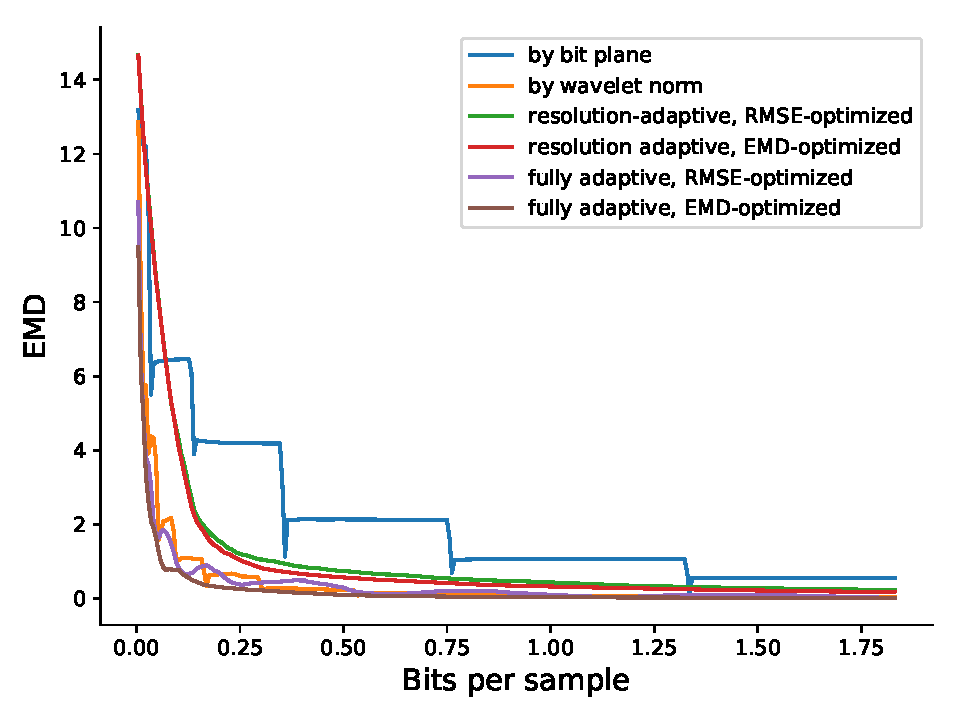
\includegraphics[width=0.44\linewidth]{img/motivation/magnetic-histogram-motivation.pdf}}
	\subcaptionbox{Boiler-O2}
	{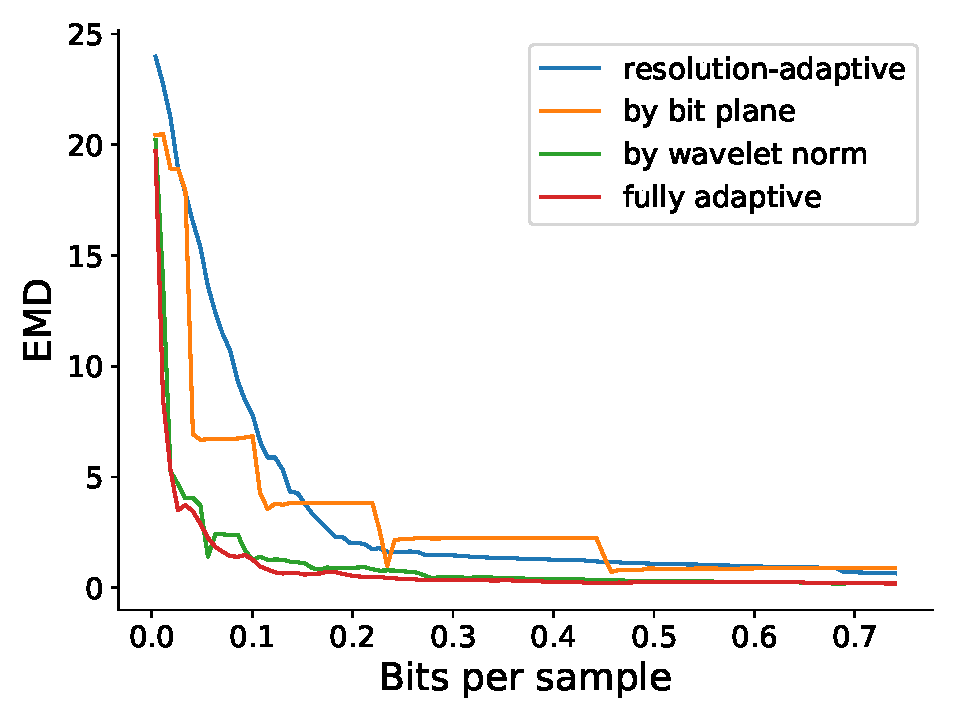
\includegraphics[width=0.44\linewidth]{img/motivation/boiler-histogram-motivation.pdf}}
	\subcaptionbox{Flame-OH}
	{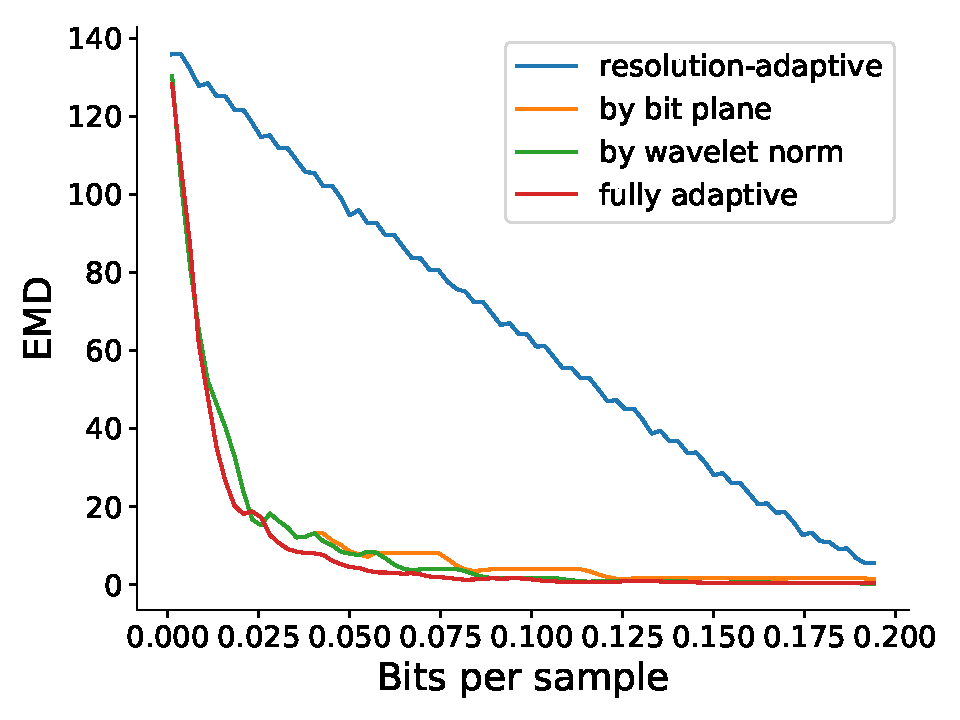
\includegraphics[width=0.44\linewidth]{img/motivation/kflame-oh-histogram-motivation.pdf}}
	\subcaptionbox{Miranda-diffusivity}
	{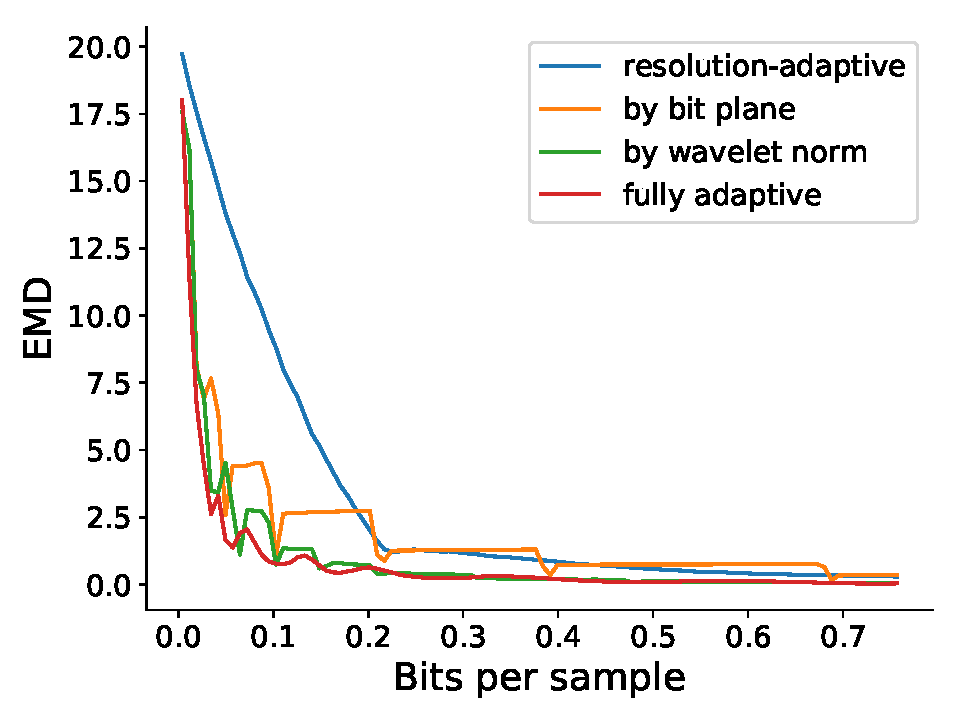
\includegraphics[width=0.44\linewidth]{img/motivation/diffusivity-histogram-motivation.pdf}}
	\caption{Histogram error comparison. Lower EMD is better. The streams are truncated	towards the
	end where the errors become negligibly small.}
	\label{fig:histogram-motivation}
\end{figure}

The \emph{by bit plane} and \emph{by wavelet norm} streams match one another closely in terms of
PSNR, but differ significantly in EMD. Furthermore, the \emph{fully adaptive, RMSE-optimized} stream
underperforms  \emph{fully adaptive, EMD-optimized}, indicating that recontructing an accurate
function and reconstructing an accurate histogram require two very different orderings of bits.
Figure \ref{fig:histogram-comparison} illustrates how a quantitative difference in EMD translates to
a visual difference in histogram.

\begin{figure}
	\centering
	\subcaptionbox{\emph{by bit plane}}
	{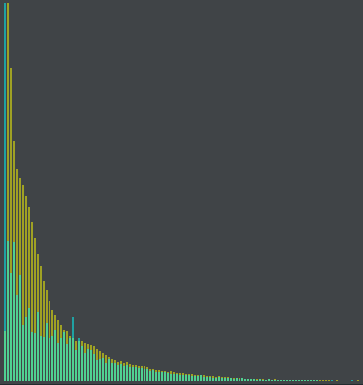
\includegraphics[width=0.24\linewidth]{img/motivation/histogram-by-bit-plane.png}}
	\subcaptionbox{\emph{by wavelet norm}}
	{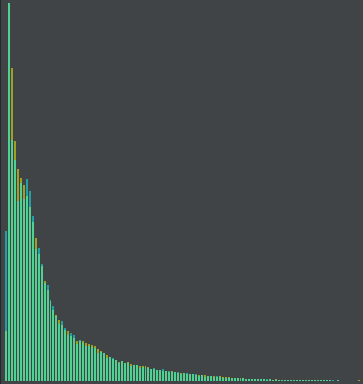
\includegraphics[width=0.24\linewidth]{img/motivation/histogram-by-wavelet-norm.png}}
	\subcaptionbox{\emph{fully adaptive, RMSE-optimized}}
	{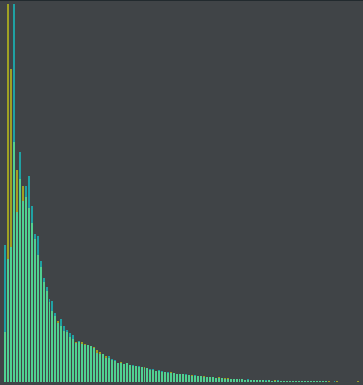
\includegraphics[width=0.24\linewidth]{img/motivation/histogram-rmse-optimized.png}}
	\subcaptionbox{\emph{fully adaptive, EMD-optimized}}
	{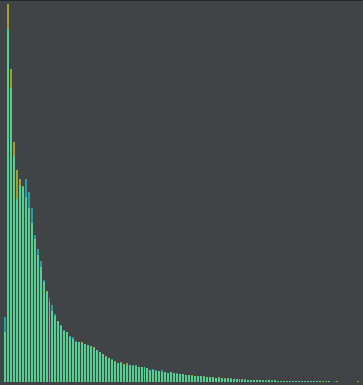
\includegraphics[width=0.24\linewidth]{img/motivation/histogram-emd-optimized.png}}
	\caption{Histogram comparison for the Magnetic data set at 0.16 bits per sample. The reconstructed
	histogram (blue) is blended with the ground truth histogram (yellow), so green is where the two
	overlap. Larger overlap (more green, less blue and yellow) is better.}
	\label{fig:histogram-comparison}
\end{figure}



\subsection{Computation}
In~\Cref{sec:combining} we demonstrated that different tasks may need different streams. For example,
PSNR stream significantly underperforms the histogram stream when applied to the histogram
query~(\Cref{fig:histogram-comparison}).
Unfortunately, there is no single definition of best stream is for a given query. It could be a stream that
exhibit small changes in the data or stream that reaches the smallest error fastest.
Moreover, it is common to stop the streaming in case the quantity of interest is good enough or the data size
reached the limit of the machine.

We define the best stream as
a sequence of refinements that reach the minimum error at given stopping bit budget. Alas, in interactive application
we can only make assumptions what will be the number of bits streamed before user decides to stop the streaming. For
example, if a user drasticly changes viewpoint in a volume rendering application, the stream starts almost from scratch.
Taking the lack of control over the stopping budget to the extreme, the best stream becomes the one which minimizes
the error at all bit budgets. However, as in any optimization problem we may reach local minimum, as
chunks that improve the error but have impact on later refinement will have lower priority. The existence of local
minima prevents this progressive stream to be globally optimal.
We can compute the optimal stream by searching the ordering space for one that is optimal for the largest number
of bit budgets. Unfortunately, finding such ordering is exponential in number of chunks. Therefore, we focus on
finding a greedy scheme that could be good representative for the optimal stream. There are two primary directions
along which we can greedily search for sream: fine-to-coarse or coarse-to-fine.

\paragraph*{Fine-to-coarse greedy algorithm} utilizes full dataset to construct the stream.
Moreover,
if we wanted to precompute stream order which could be utilized during query, we would have access to whole
data set and could compute this stream. The algorithm is in principle a reverse of the previous approach, the
stream is constructed by starting with full data set and one by one disabling the chunks. At each step, a chunk
with smallest errorr impact is disabled (TODO: more detail). This algorithm is still of greedy nature as it
makes only locally optimal choice.
The running time of this algorithm is $O(n^3)$ as we start with $n$ chunks
and at each streaming step decrease the chunk count by one. The cube factor comes from the need to perform inverse
wavelet transform and compute the error for each chunk.

\begin{algorithm}
  \KwData{slice, unordered list of chunks}
  \KwResult{ordered list of chunks with decreasing error}
  orderedChunks = $\emptyset$\;

  \While{$|$chunks$| \ne 0$}{
   smallestChunk = front(chunks)\;
   \For{chunk $\in$ chunks}{
     sliceCopy = slice\;
     disableChunk(sliceCopy, chunk)\;
     error = computeError(sliceCopy, slice)\;
     \If{error $<$ error(smallestChunk)}{
       smallestChunk = chunk\;
     }
   }

   disableChunk(slice, smallestChunk)\;
   chunks = chunks $\setminus$ smallestChunk\;
   orderedChunks = orderedChunks $\cup \{$smallestChunk$\}$\;
  }
  \caption{Fine-to-coarse stream optimization algorithms}
\end{algorithm}

\begin{figure}
        \centering
        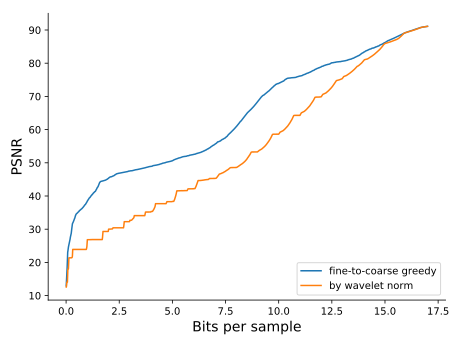
\includegraphics[width=0.48\linewidth]{img/figure4_new/rmse-miranda-viscosity}
        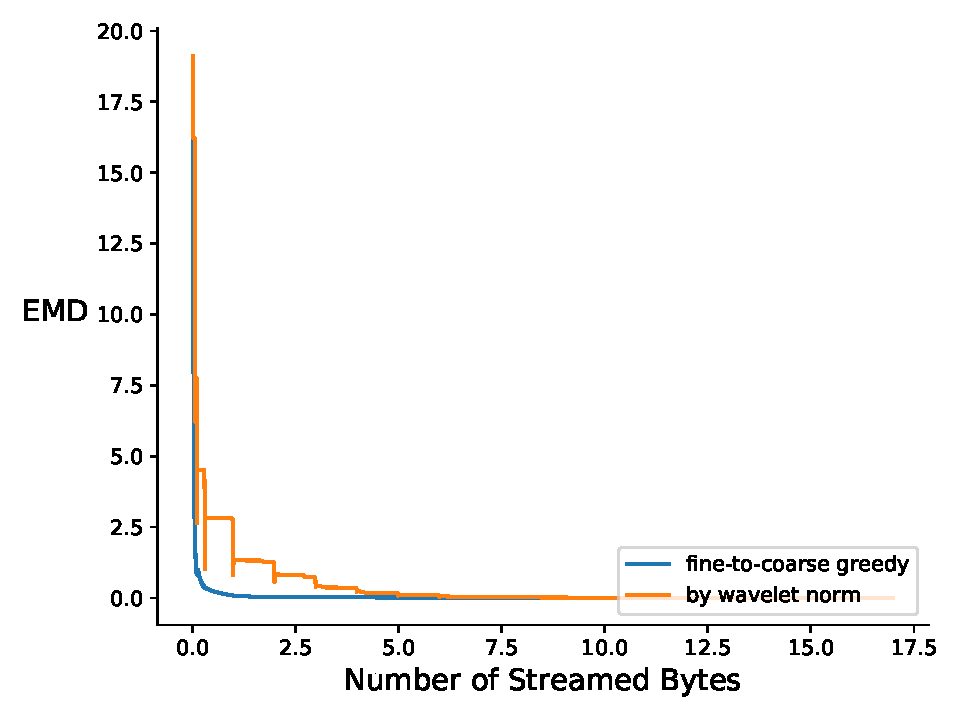
\includegraphics[width=0.48\linewidth]{img/figure4_new/histogram-miranda-viscosity}
        \caption{Comparison of fine-to-coarse and by wavelet norm streams on Miranda viscosity data set.
                 On the left is stream optimized for PSNR (higher is better) and on the right for histogram (lower is better).
                 Despite using larger block size for the greedy stream ($16 \times 16$) due to performance reasons, it still
                 significantly outperforms the by wavelet norm stream for both quantities.}
\end{figure}


\paragraph*{Coarse-to-fine greedy algorithm} starts with no data and
the initial error is computed with respect to the full data set. Then
it takes a list of all chunks in the dataset, computes the error as if
the chunk was enabled, and picks the chunk with the highest absolute
difference in the error with respect to the current error.  We use
absolute difference to avoid the case where the error difference is
zero or negative, which would result in a long stream of chunk that do
not decrease the error significantly. \ptb{I am not sure in understand
  the previous sentence} This assumption reflects the expectation of
more data meaning better result. Similarly to the coarse-to-fine
algorithm, the running time is still $O(n^3)$.


Since the fine-to-coarse greedy stream outperforms the coarse-to-fine stream we further investigate possible
runtime optimizations. Surprisingly, performing only the first round of chunk error calculation and then sorting
those chunks by the error closely matches the full greedy algorithm. This simple optimization reduces the time
complexity to $O(n^2)$ and thus makes it more practical. We use this greedy scheme throught our evaluation named
\emph{fully adpative} stream.

\begin{figure}
        \centering
        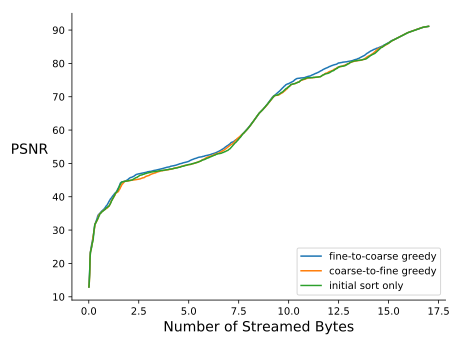
\includegraphics[width=0.48\linewidth]{img/figure6/rmse-miranda-viscosity}
        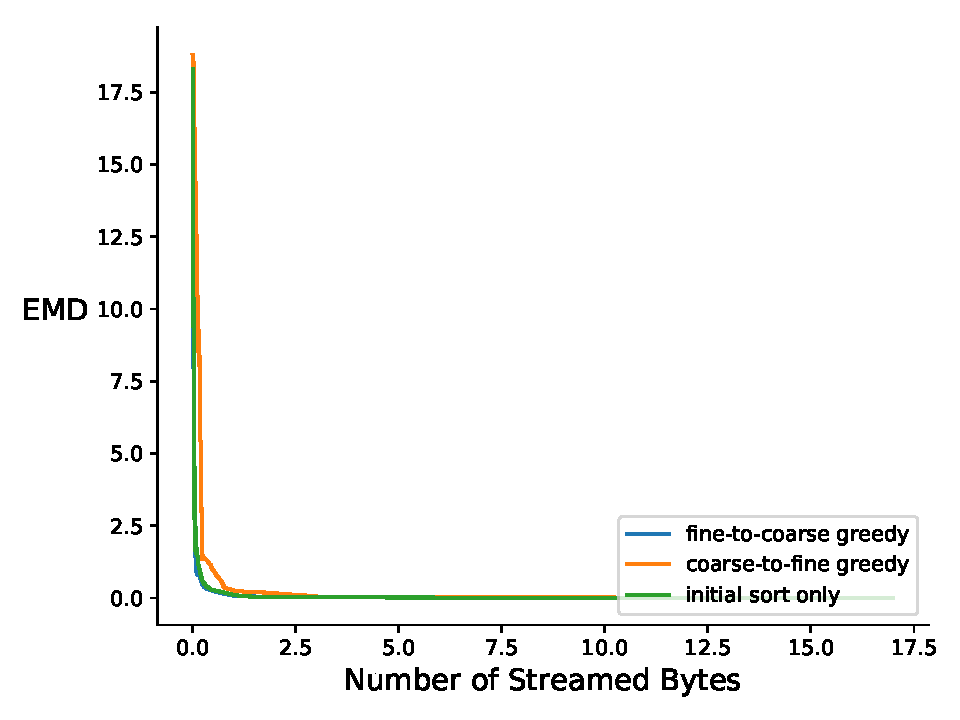
\includegraphics[width=0.48\linewidth]{img/figure6/histogram-miranda-viscosity}
        \caption{The fully adaptive stream (fine-to-coarse with only initial sorting) closely follows the coarse-to-fine and
                 fine-to-coarse streams both for PSNR and histogram.}
\end{figure}

%%% Local Variables:
%%% mode: latex
%%% TeX-master: "template"
%%% End:

\section{Observations}
TODO: do we show visualization from the tool?

Introduce the concept of ``signature'' as a way to quantify the relative ordering of bits belonging to different bit planes and subbands (but in the same spatial region).

Figure: example signature of a stream

Algorithm: how to compute signature for a stream

%To demonstrate that this ``signature'' concept is meaningful, we construct ``hybrid'' streams as follows. Suppose we have stream-isocontour and stream-rmse for the same data. We construct stream-hybrid1 by following stream-rmse in terms of ordering of regions, while following stream-isocontour within each region by using its signature. Also construct stream-hybrid2 by following stream-isocontour in terms of ordering of regions and stream-rmse within each region. Yet another hybrid is stream-hybrid3 that follows stream-isocontour both in ordering of regions and within each region. Comparing these streams in terms of isocontour error, we will see stream-isocontour > stream-hybrid3 > stream-hybrid2 > stream-hybrid1 > stream-rmse. This means the concept of signature is meaningful.

\subsection{Comparing gradient, Laplacian and rmse streams}
NOTE: for these we use the b-spline 4-4 wavelets which have four vanishing moments so that the reconstructed function is smooth enough for taking derivatives

Figure 1: gradient difference between gradient and rmse streams

Figure 2: Laplacian difference between Laplacian and rmse

Figure 3: PSNR plot for gradient, laplacian and rmse streams

Figure 4: visual comparison of gradients and laplacian at low bit rate

Figure 5: signature comparing the three streams

We conclude that the rmse strea subsumes gradient and laplacian

\subsection{comparing isocontour and rmse}
Figure 1: show signatures of the two streams

We compute the hybrid stream that follows the isocontour stream in terms of regions, but within each region, follows the rmse stream.

Figure 2: a plot comparing the rmse, isocontour, and hybrid in terms of isocontour error. We observe that the hybrid is close to the isocontour stream.

figure 3: show isocontour rendering for the three streams at some low bit rates where the errors are apparent. Ideally the difference between isocontour and hybrid is not noticeable.

%figure 4:  Suppose we have stream-isocontour and stream-rmse for the same data. We construct stream-hybrid1 by following stream-rmse in terms of ordering of regions, while following stream-isocontour within each region by using its signature. Also construct stream-hybrid2 by following stream-isocontour in terms of ordering of regions and stream-rmse within each region. Yet another hybrid is stream-hybrid3 that follows stream-isocontour both in ordering of regions and within each region. Comparing these streams in terms of isocontour error, we will see stream-isocontour > stream-hybrid3 > stream-hybrid2 > stream-hybrid1 > stream-rmse. This means the concept of signature is meaningful.

Figure 4:
Here, using a synthetic data set (gaussian function) we compare the signature of three isocontour streams at different isovalues, where the derivatives of the function are: low, medium, high. We will observe different orderings (signatures) in each case.

\subsection{Comparing histogram and rmse}
Figure 1: show signature of the two streams

Figure 2: show comparison of histograms using different number of bins and rmse in terms of PSNR

Figure 3: plot histogram error of rmse and histogram streams and show visually the different histograms at some low bit rate.

Figure 4: Show that we can stream using the histogram signature to get better histogram than rmse
\section{Conclusion}

We presented a study of tradeoff between resolution and precision for commonly used derived
scientific quantities such as RMSE, gradient, Laplacian, histogram, and isosurface.
During this study, we covered the gamut of scientific data sets, ranging from simulations
with smooth features or fine scale detail to image data with noisy parts\pavol{do we have plot of image data?}.
We showed that one stream type does not fit all analysis tasks, but some streams perform well
in most of them and may be useful in a new file format design.

We started with an evaluation of contemporary techniques for reducing resolution or precision.
The experiments showed that streaming only in resolution or precision is suboptimal for all
tested queries. We thus developed a tractable greedy algorithm for computing adaptive stream order
based on the particular task. The produced stream significantly\pavol{it would be good to quantify what
significantly means, 2x?} outperforms any stream that has
a fixed streaming order.

After establishing the greedy algorithm for computing a stream, we focused on each query and
investigated which queries have similar streams. This approach is important because if two streams
are very similar, we can precompute the stream order and apply the same ordering to different
queries.

For example, we learned that the RMSE stream is akin to the gradient stream, and thus only one
needs to be computed. Moreover, since RMSE optimizes for the function, the stream alongside
a good gradient approaches the function itself. In contrast, the gradient ignores the constant offest
of all samples, resulting in an inferior RMSE.


These results should be considered when designing a file format for scientic data. As future work,
we plan to create new file format that will incorporate the stream-ordering techniques we presented.
Additionally, such file format needs to support compression and spatial adaptivity to handle large-scale
data and fast queries. We are investigating if signatures can be used to handle
the spatial adaptivity. For example, we could extend the signature matrix to the tensor, with
the spatial index being the third dimension.

\end{document}
